% !TEX root = ../main.tex
\section{Perceptual Ambiguity}
\label{sec:problem}
In most square fiducial tag detection, the pose is calculated by fitting a quad around the planar tag. The corners are extracted from the tag and the pose is estimated using 3D to 2D point correspondence optimization methods such as Levenberg–Marquardt [OpenCV reference] or DLT. This is a specific case of the perspective-n-point problem and it has been well studied in geometry based Computer Vision literatures [][]. In particular, there is a deterministic solution to the perspective-4-point problem. In other words, given the projection of a tag corners, the pose of the tag is unique. In reality, however,  when a small tag is captured in a low resolution camera, the perspective projection becomes almost orthographic. In these cases, a small variance in the corner detection process will yield estimations far from the true pose due to a perceptual ambiguity under projection. 

We will illustrate this effect by using two over lapping cubes in figure 3. The overlapping face of the two cubes are interlaced but rotated by 120 degrees. However, due to perspective projection the squares appears to be on the same plane. Under low camera resolution, the over lapping squares become virtually indistinguishable. The red circular regions are the detected corners under some sensory noise. In these cases, the optimal PnP solution is no longer singular but a bimodal distribution depending on the viewing angle. The result of the 3D to 2D correspondence optimization might return either one of the two solution.
\begin{figure}
\centering
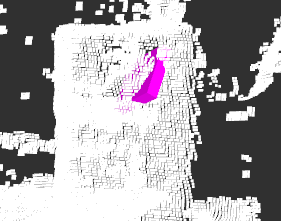
\includegraphics[width=\columnwidth]{figs/mismatch_tag}
\caption{The orientation of Apriltag placed on the object is greatly misaligned with the actual object}
\label{fig:calib}
\end{figure}

\begin{figure}
\centering
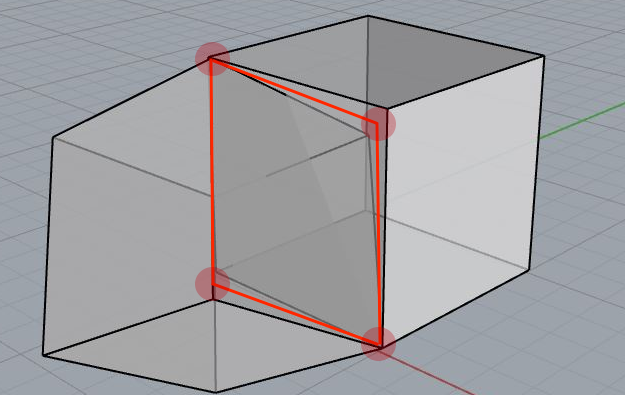
\includegraphics[width=\columnwidth]{figs/perspective_fig}
\caption{Perspective Ambiguity illustrated with overlapping cubes}
\label{fig:calib}
\end{figure}